\section{Findings}

We report participants’ perceptions of the AI guide, the guide’s accuracy across tasks, and how participants behaved towards the guide in solo and social settings.

\subsection{Overview}
All participants explored both parks and attempted to provide tours. While describing the parks to the confederates, all participants provided accurate information about the parks, demonstrating that they had learned the park contents. However, providing a tour proved more challenging: 10 out of 16 participants met the requirement of guiding their group to two landmarks, three guided them to more than two, and six made it to one. Participants who struggled with this task often forgot the names of landmarks and that they could give the guide descriptions of desired landmarks instead of names to trigger guidance.

Other participants struggled due to inaccuracies made by the guide. While the guide responded correctly to a total of 301 out of 476 queries (63.2\%), factors such as misinterpreting participant accents or receiving incomplete queries from participants reduced guide accuracy. When responding to requests, the guide’s average response time was 6.1 seconds for guidance requests, 11.2 seconds for visual questions, and 6.8 seconds for interpersonal queries.  We categorized queries into seven request types: navigation (e.g., “Take me to the fountain”), visual description (e.g., “Describe the structure in front of me”), clarification (e.g., “Could you repeat what you said? I didn’t understand.”), audio beacon (e.g., “Put an audio beacon on the northern gazebo”), social interaction (e.g., “Say ‘hi’ to my friends here, Giddy”), confirmation (e.g., “I’m looking at a patch of flowers, right?”), and auditory description (“What’s making that watery sound?”). Of these types, navigation and visual interpretation were most common, making up 60.4\% and 31.4\% of requests, respectively.

When conversing with the guide, participants typically spoke with a utilitarian tone (see Figure \ref{fig: request_tone}), with 74.6\% of interactions being straightforward and commanding (e.g., “Take me to the fountain”). 15.8\% were polite (e.g., “Could you please take me to the fountain?”) and 9.6\% of remaining interactions were friendly (e.g., “Hey buddy, let’s go to the fountain”).

Though we did not explicitly compare participants’ experience with the two guide personas they used–the guide dog and robot–we did note differences in how they initially reacted to each. The dog persona was generally thought of as “cuter” (Anika, Niya) or more “empowering” (Aiden, Nikolai, Xiran), due to it being a symbol of blindness. Participants also demonstrated different behaviors towards the guide depending on its persona, which we detail in section \ref{sec: Behavior Towards the Guide}.

\begin{figure}
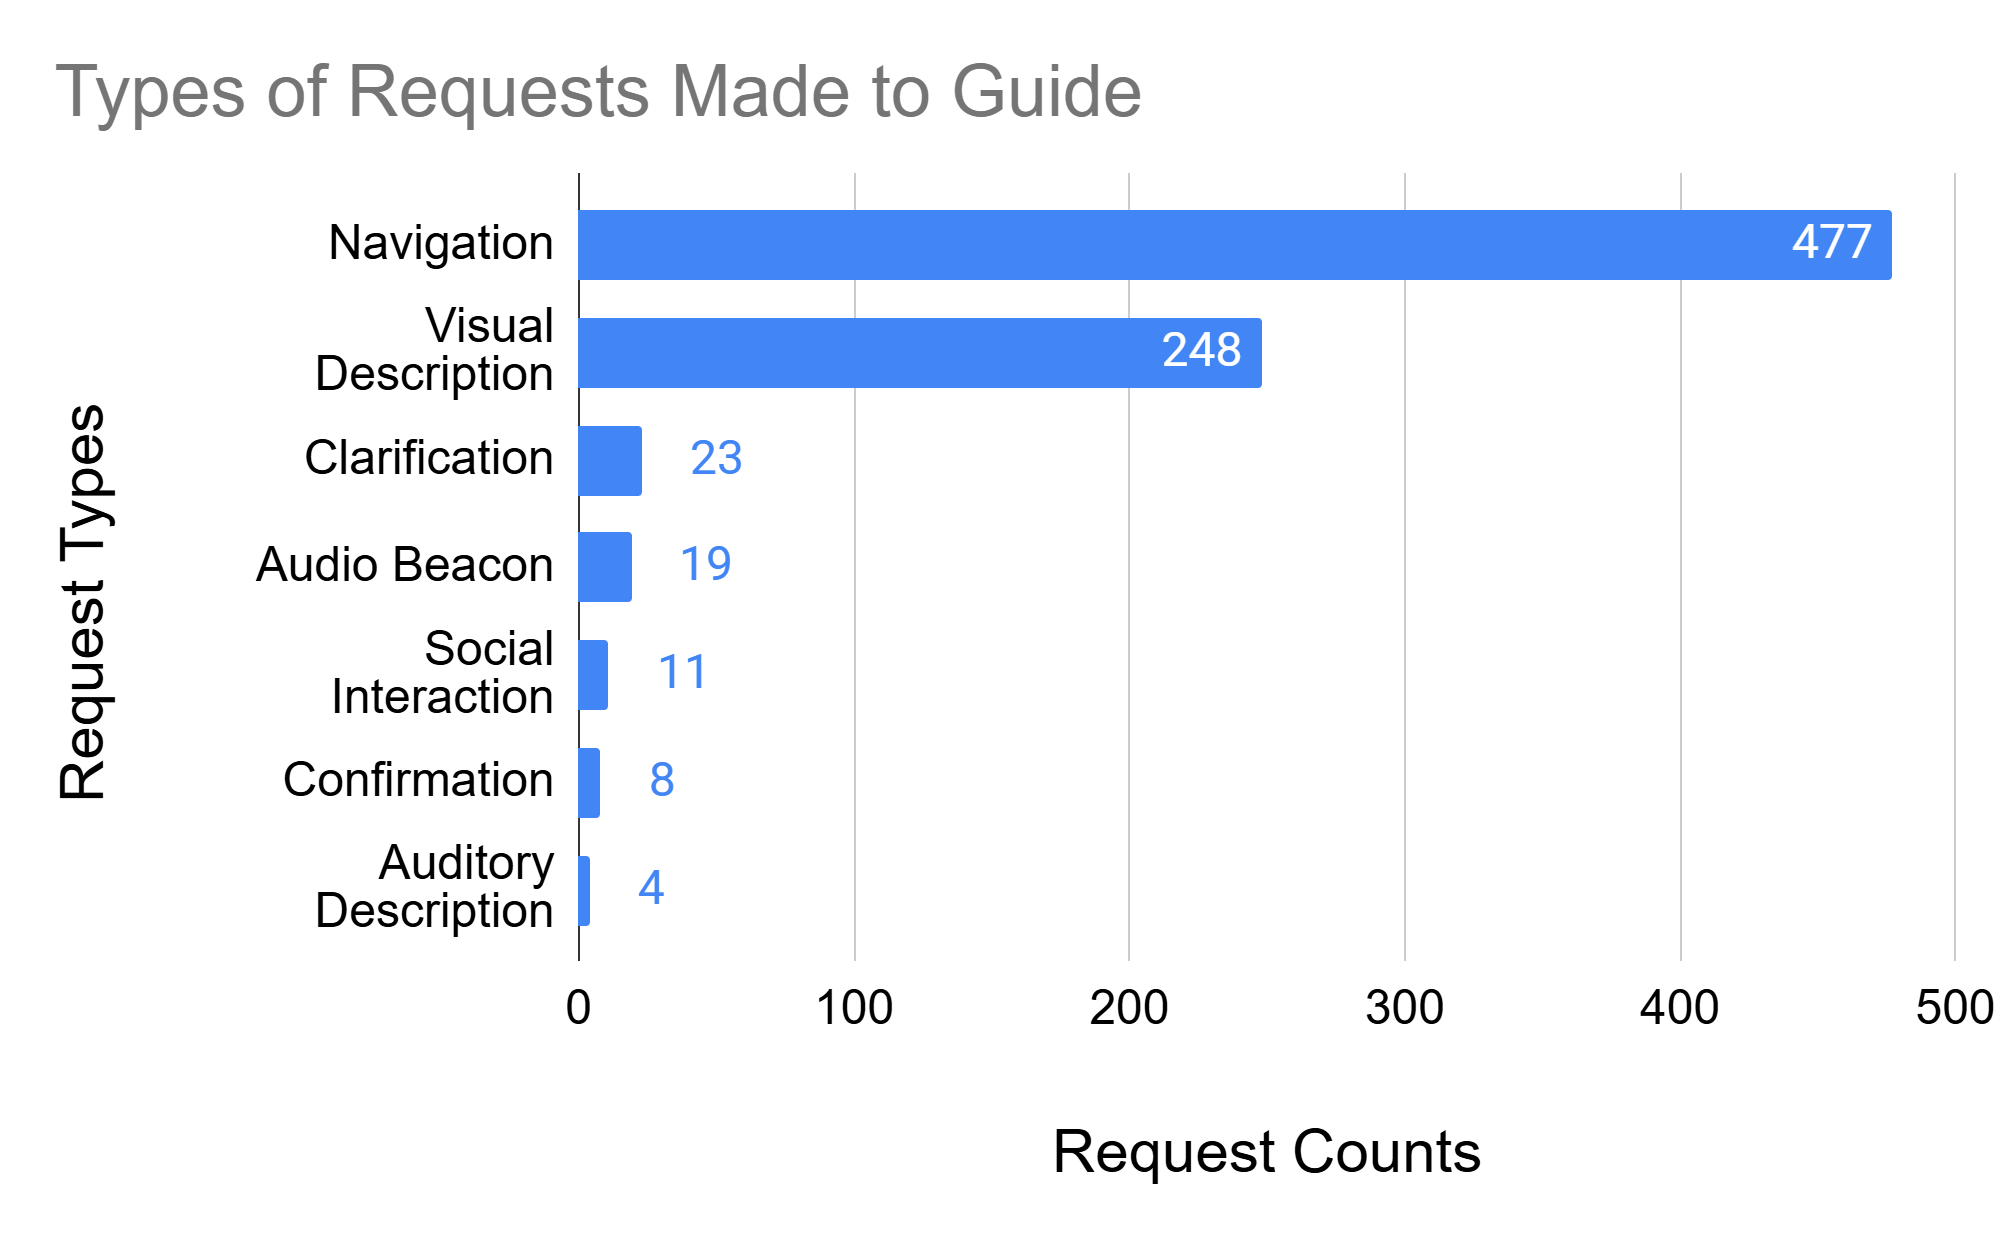
\includegraphics[width=250pt]{request_type.png}
\caption{\label{fig: request_type} Types of requests made to the guide. Participants made a total of 799 individual requests within 467 user queries, as many queries encompassed multiple request types. For instance, the query “Describe where that sound is coming from” includes both a visual description and an auditory description.
}
\Description{A bar chart depicting the types of requests users made to the guide.

The bar chart is titled "Types of User Requests Made to the Guide." It shows seven categories on the vertical axis labeled "Request Types", and runs from 0 to 500 on the horizontal axis labeled "Request Counts." In order from top to bottom, and greatest to least, the bar chart shows bars for: "Navigation" (477 requests), "Visual Description" (248 requests), "Clarification" (23 requests), "Audio Beacon" (19 requests), "Social Interaction" (10 requests), "Confirmation" (8 requests), and "Auditory Description" (4 requests).
}
\end{figure}
\begin{figure}
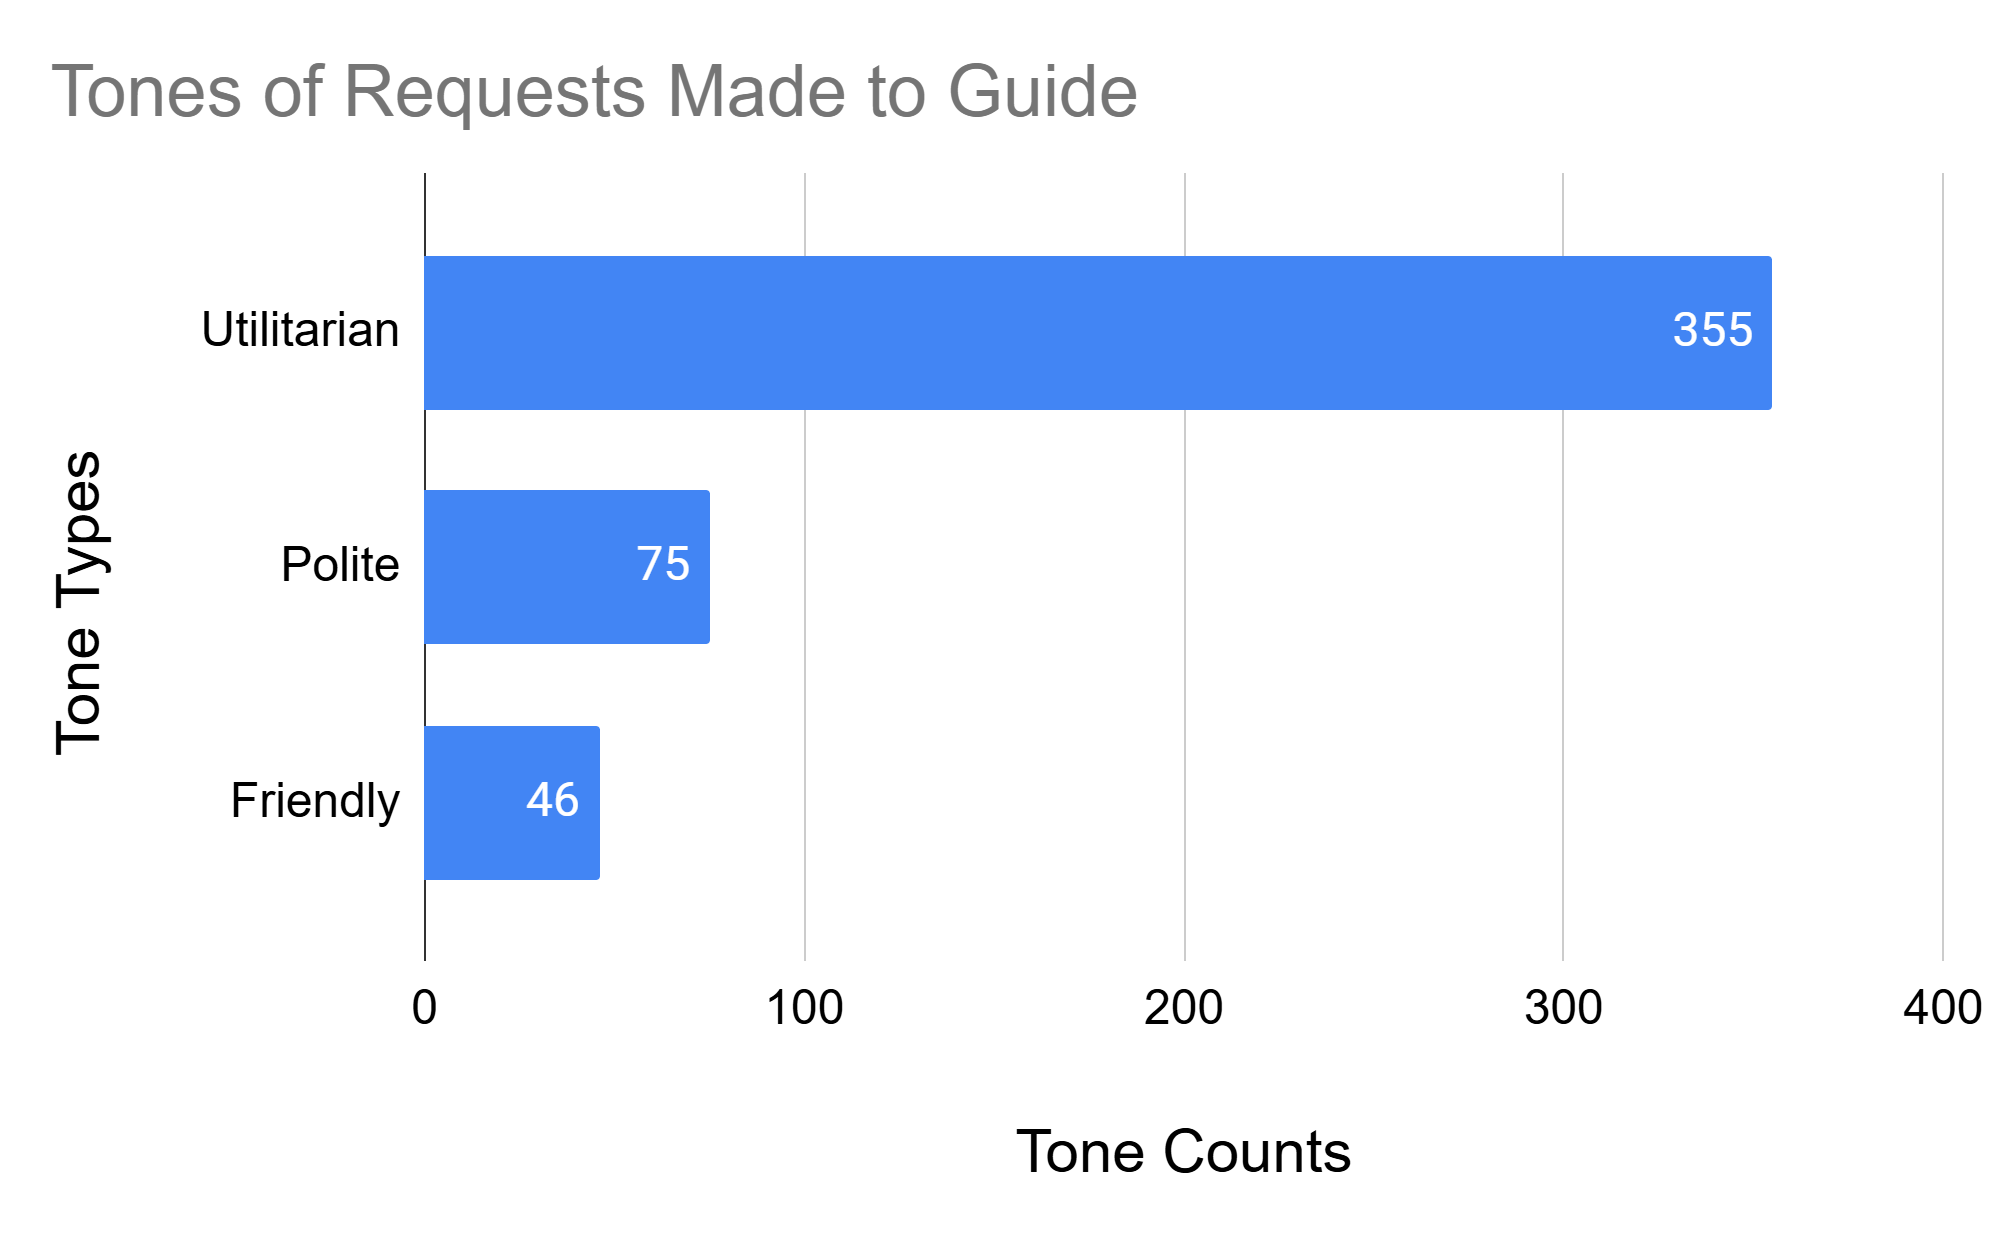
\includegraphics[width=250pt]{request_tone.png}
\caption{\label{fig: request_tone} Tones of requests made to the guide. Participants made 476 requests total, one for each query to the guide, as each query counted as a separate utterance with its own tone.}
\Description{A bar chart depicting the different tones of requests users made to the guide.

The bar chart is titled "Tones of Requests Made to the Guide." It shows three categories on the vertical axis labeled "Tone Types", and runs from 0 to 400 on the horizontal axis labeled "Tone Counts." In order from top to bottom, and greatest to least, the bar chart shows bars for: "Utilitarian" (355 requests), "Polite" (75 requests), and "Friendly" (46 requests).
}
\end{figure}

\subsection{Participants’ Ratings of the Guide and their VR Experience}

We present participants’ assessments of the guide based on Likert scale scores reported in Figure \ref{fig: request_tone}. We do not include feedback from three participants (Li, Yadriel, Jiwoo) who did not use the guide. However, their experiences are described in section \ref{sec: Completing Tasks Without The Guide}.

\begin{figure*}[t]
\centering
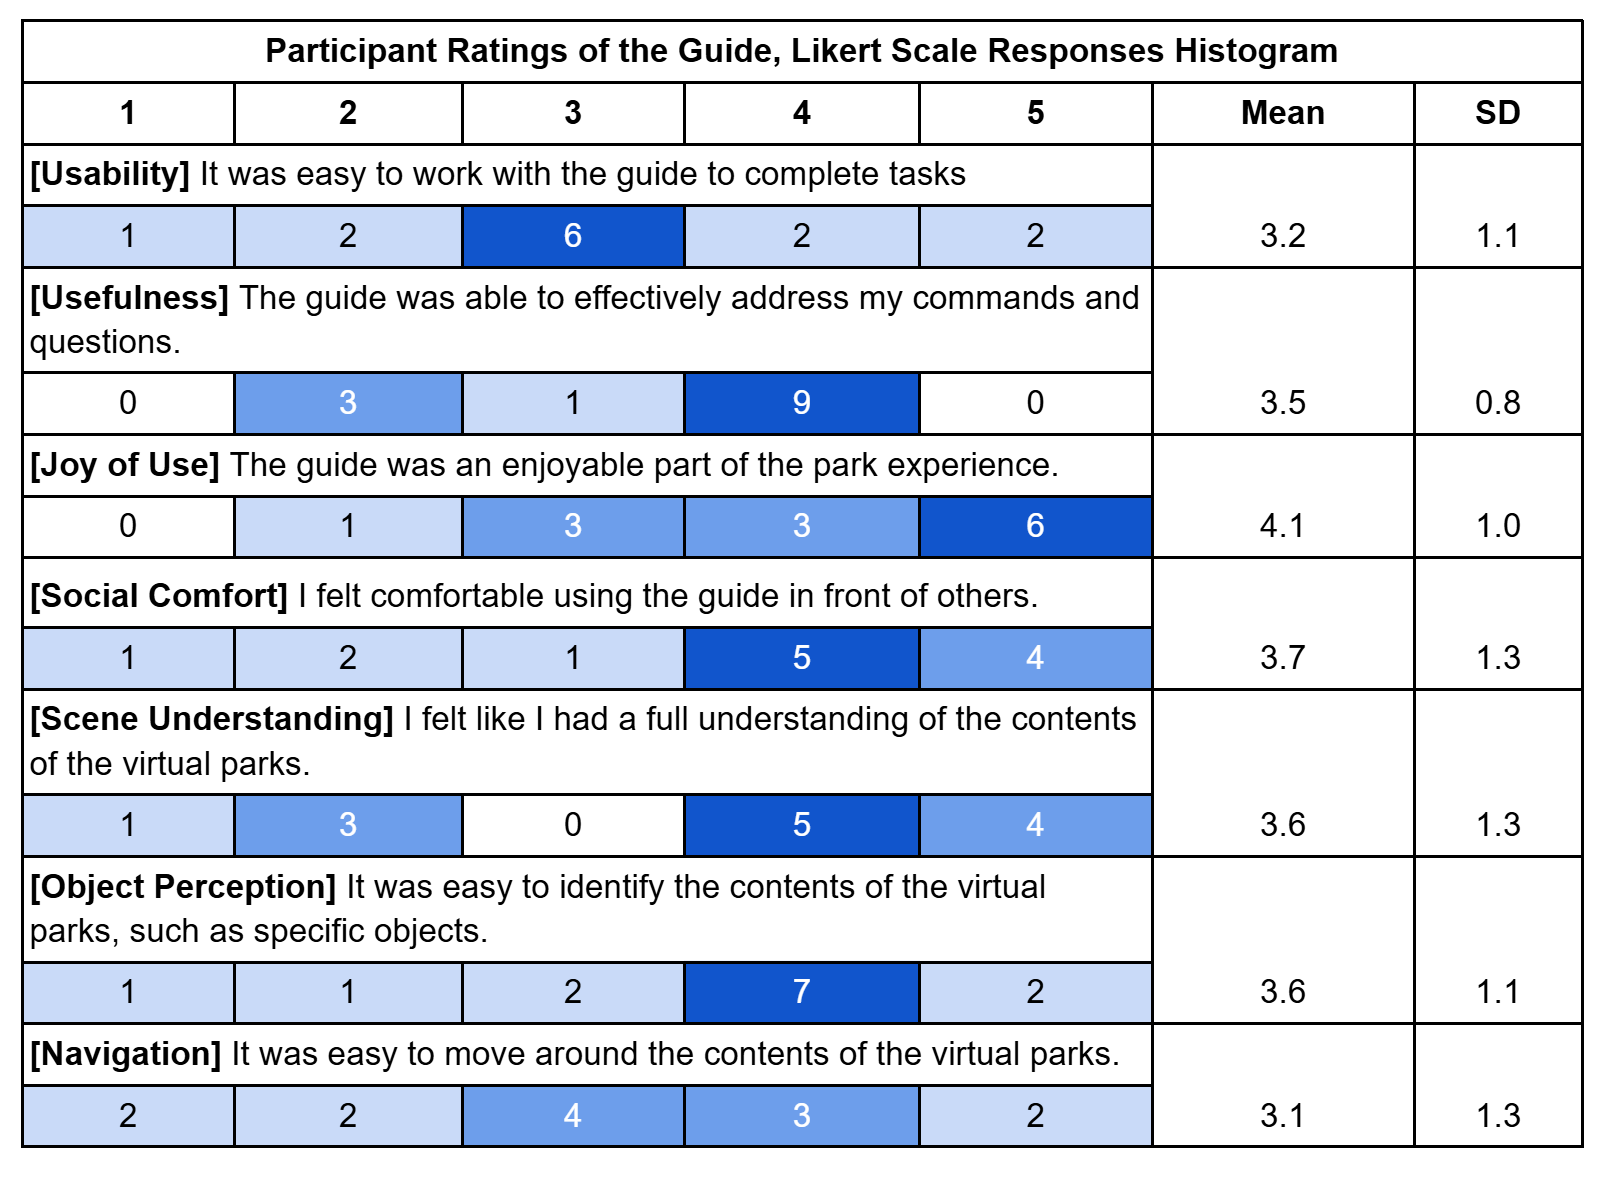
\includegraphics[width=350pt]{likert_responses.png}
\caption{\label{fig: Likert Guide Ratings} Likert scale responses from participants rating the guide, collected after participants experienced both parks and guide personas. Scores were given on a scale of 1 to 5, where 1 = strongly disagree, 2 = disagree, 3 = neither agree nor disagree, 4 = agree, and 5 = strongly agree. Note: In the statement on Social Comfort, “others” refers to the confederates participants met during the study. We only include scores from thirteen participants who used the guide.
}
\Description{A histogram containing the Likert-scale response data from participants rating the guide on various qualities. The scale runs from 1 to 5, with numbers in columns below depicting how many responses from participants fell under each number on the scale for a given statement and factor. They are colored in various shades of blue, with the darker colors representing more responses falling under a particular number on the scale and the lighter colors representing fewer.

For the statement: [Usability] It was easy to work with the guide to complete tasks.
The histogram reports 1 user responded 1, 2 users responded 2, 6 users responded 3, 2 users responded 4, and 2 users responded 5. The mean is 3.2, standard deviation 1.1.

For the statement: [Usefulness] The guide was able to effectively address my commands and questions.
The histogram reports 0 users responded 1, 3 users responded 1, 1 user responded 3, 9 users responded 4, and 0 users responded 5. The mean is 3.5, standard deviation 0.8. 

For the statement: [Joy of Use] The guide was an enjoyable part of the park experience.
The histogram reports 0 users responded 1, 1 user responded 2, 3 users responded 3, 3 users responded 4, and 6 users responded 5. The mean is 4.1, standard deviation 1.0. 

For the statement: [Social Comfort] I felt comfortable using the guide in front of others.
The histogram reports 1 user responded 1, 2 users responded 2, 1 user responded 3, 5 users responded 4, and 4 users responded 5. The mean is 3.7, standard deviation 1.3. 

For the statement: [Scene Understanding] I felt like I had a full understanding of the contents of the virtual parks.
The histogram reports 1 user responded 1, 3 users responded 2, 0 users responded 3, 5 users responded 4, and 4 users responded 5. The mean is 3.6, standard deviation 1.1. 

For the statement: [Object Perception] It was easy to identify the contents of the virtual parks, such as specific objects.
The histogram reports 1 user responded 1, 1 user responded 2, 2 users responded 3, 7 users responded 4, and 2 users responded 5. The mean is 3.6, standard deviation 1.1. 

For the statement: [Navigation] It was easy to move around the contents of the virtual parks.
The histogram reports 2 users responded 1, 2 users responded 2, 4 users responded 3, 3 users responded 4, and 2 users responded 5. The mean is 3.1, standard deviation 1.3. 

}
\end{figure*}

\textbf{Usability}. Four participants somewhat or strongly agreed that it was easy to work with the guide to complete tasks, noting that the controls were straightforward and the guide generally understood their queries (mean 3.2, SD = 1.1). For instance, Nikolai appreciated the ability to activate the guide without needing to know its exact location. Conversely, nine participants disagreed or felt neutral about the guide’s usability, reporting difficulties with controls.

Some participants (Niya, Maritza, Siobhan) found the guide's inconsistent response style challenging. Though inconsistency is a common quality of AI-generated content, where the AI changes how it replies so as to sound more natural, this quality was not helpful in a guidance context, especially for participants used to the consistent manner of communication typical of human guides. Siobhan remarked that she wished “the directions maybe, could be consistent each time, so that they are not quite as abstract, and they don't vary quite as significantly every single time.”

Other participants (Xiran, Aiden, Len, Jamal) expressed that the guide struggled to comprehend nuanced instructions. Xiran wanted the guide to bring her on a continuous tour around the park, moving from one landmark to another. However, when she attempted to prompt the guide for such navigation, it instead provided generic verbal directions like “walk straight” (Xiran). Similarly, Len tried to prompt the guide to go to a previously mentioned flower patch with slightly poetic language, saying: “Let’s go smell the flowers.” In response, the confused guide gave a description of the nearest flowers: “Smelling flowers sounds splendid! There are several vibrant flower patches around, each bursting with color and light…”

\textbf{Usefulness}. Despite usability challenges, nine participants found the guide useful, somewhat agreeing that it was able to address their commands and questions (mean 3.5, SD = 0.8). They commented that the guide felt “necessary” (Teo) to experience VR, and that it allowed them to get more information than “randomly exploring” (Anika) on their own would have.

\textbf{Joy of Use}. Nine participants enjoyed using the guide, somewhat or strongly agreeing that the guide was an enjoyable part of their experience (mean 4.1, SD = 1.0). Other participants were more neutral, feeling that it did not have to be enjoyable since it was an assistive tool (Jamal) or that enhancements were needed before they considered it enjoyable (Niya, Len, Siobhan). Len, for instance, expressed a desire for greater privacy when using the guide in social settings:

\begin{quote}
I would like the guide to just be something that only I can see and hear if I'm going to be using it in a social environment. I'd like to have [a] button…that mutes my chat with everyone else around me, so the only thing that's hearing me is my guide…For lack of a better term, [an] introvert guide setting where I could just be like, ‘Alright. This is \textit{my} guide for \textit{me} to see.’ …[that I could turn] on and off.
\end{quote}

\textbf{Social Comfort}. Nine participants reported feeling comfortable using the guide in front of other people (mean 3.7, SD = 1.3). They attributed their comfort to prior experiences using assistive devices. Aiden elaborated: 

\begin{quote}
I'm so used to… having a guide dog or a cane, and just explaining…to people ‘I'm blind…I've attended conferences with a guide dog before. So I think just having [the guide] is just going to be like, ‘Yeah, this is my assistant and he's helping me around.’ I think I'd be comfortable with that in pretty much any situation.
\end{quote}

However, four participants expressed discomfort, primarily due to the guide's visibility to others. Despite their familiarity with visible mobility aids in the physical world, they preferred to control how and when their disability was disclosed in VR. Len remarked:

\begin{quote}
I'm not going to want [others] to know that I'm blind or visually impaired right away. It kind of blows away the anonymity of the virtual world…and the way I want to present myself…I don't want to give away certain details about myself, [even] something minuscule like my visual impairment.
\end{quote}

Others (Niya, Sara) found the guide's lingering presence “awkward” (Niya) when not actively in use. Sara noted that this feeling was mitigated when using the dog guide, since the confederates seemed to like petting and interacting with it, but it still made her uncomfortable.

Finally, participants had mixed opinions on three key aspects of their ability to explore virtual scenes: scene understanding, object perception, and navigation.

\textbf{Scene Understanding}. Nine participants somewhat or strongly agreed that they had an accurate understanding of the scene (mean 3.6, SD = 1.3). Other participants struggled with this aspect, and some (Niya, Siobhan) wanted the guide to use cardinal directions more consistently, since switching between descriptions like “north and south…then bottom or left” (Niya) was confusing.

\textbf{Object Perception}. Nine participants somewhat or strongly agreed that it was easy for them to identify virtual objects (mean 3.6, SD = 1.1). Others found object perception more challenging, and some (Xiran, Len) commented that the guide did not improve their perception abilities. They explained that the guide’s descriptions of objects were “passable” (Xiran), but did not make them feel confident that they understood what they were looking at.

\textbf{Navigation}. Five participants somewhat or strongly agreed that it was easy to move around the parks (mean 3.1, SD = 1.3). Conversely, eight participants disagreed or felt neutral about their navigation abilities. Some participants (Aiden, Siobhan, Jamal) again referenced difficulties with the guide’s inconsistent descriptions, which did not help them build reliable “mental maps” (Siobhan, Jamal). Others (Niya, Anika, Teo, Maritza, Len, Jamal) experienced usability issues when attempting to navigate with the guide, such as forgetting the button to grab it.

\subsection{Completing Tasks with the Guide}
\label{Participant Strategies for Completing Tasks}

We report strategies for how participants approached the study tasks with the guide, in solo and social settings.

\subsubsection{Exploring Alone} \label{sec: Exploring Alone}

During solo park exploration, all participants used the guide to navigate and become familiar with park content, employing the guide in particular ways to achieve these goals. For navigation, all participants combined the guide’s abilities with their own, sometimes asking the guide to take them to different places, and other times walking or teleporting around the park themselves. To familiarize themselves with the park, nearly all participants (n = 10) posed brief questions to the guide when they needed information, such as asking for the names of objects as they encountered them. Several others (Anika, Teo, Nikolai, Xiran, Yuki, Maritza, Aiden, Len, Siobhan) used the guide to provide an overview of their environment, then chose individual details to explore further. For instance, after Yuki wandered off the path he had been following in one park, he called the guide to get his bearings again:

\begin{quote}
	\textbf{Yuki: Okay. And what's around me?}\\
Guide: You're surrounded by various things. The Red-Roofed Gazebo, the Pine Tree by the River, and more pine trees to your left. To your right is the Boat, and beyond that is the Dock–\\
Yuki: Oh, okay.\\
Guide: –To explore more of the scene, head onto the path beside the bench leading to Western Bridge. To your left, the Puffy Tree by the Bench provides some shade.\\
\textbf{Yuki: Take me to the bridge.}\\
Guide: Okay. Grab onto me, and I'll take you to Western Bridge.
\end{quote}

\subsubsection{Leading Others to Landmarks} \label{sec: Leading Others to Landmarks}

While exploring on their own, participants occasionally walked and teleported by themselves; however, during the group tours, they always used the guide to lead their group between landmarks. Participants used the guide to lead their groups in two ways. More commonly, they ordered the guide to take them to identified landmarks, and asked the confederates to follow them. Less commonly, they asked for an audio beacon or the guide misinterpreted their request and placed an audio beacon on a landmark. In this case, participants walked towards the sound of the beacon to lead their group, as Aiden did in the following exchange:

\begin{quote}
Aiden: Welcome to the park. I'm your tour guide for the day. So is there, is there anything you would like to see?\\
Confederate 1: I mean, if you have a favorite part of this park to take us to, then we can go there.\\
Aiden: Yeah, I kind of like the north platform there, where you can kind of see a lot of the different stuff around. So let's walk over there.\\
Confederate 1: Alright.\\
Confederate 2: That sounds cool.\\
\textbf{Aiden: Okay.} \textit{[To the guide]} \textbf{Walk me to the northern platform.}\\
Guide:  Very well. I will add an audio beacon to Northern Platform.\\
\textbf{Aiden:}  \textit{[To the confederates]} \textbf{Alright. So if you guys will follow me here, I'll walk up there.}
\end{quote}

\subsubsection{Filling Gaps in Knowledge} \label{sec: Filling Gaps in Knowledge}

Throughout the tours, participants used the guide to help them answer confederates’ questions. Typically, they first responded to questions based on what they had learned themselves during solo exploration. However, if participants needed additional information to answer fully, they called the guide. In the following conversation, Sara realized she had forgotten an important detail about the park as she was describing it:

\begin{quote}
\textbf{Sara:} Okay. So right now, we're on this dock. There's a boat in front of us. Nice little river running past the bridges. \textbf{There is one, two, so there's a, oh, boy! What is that called again? One second.} \textit{[To the guide]} \textbf{What is this structure?}\\
Guide: You are looking at the Orange-Roofed Gazebo.\\
\textbf{Sara: Oh, gazebo!} \textit{[To the confederates]} \textbf{I've never heard of that word before.} So there's an orange gazebo, a red gazebo, and a yellow gazebo.
\end{quote}

Maritza also used the guide to answer confederate questions, not to recall forgotten information, but to obtain details she had never learned:

\begin{quote}
Confederate 1: How big is this place?\\
\textbf{Maritza:} All right. Let's all go to the, oh. \textbf{We are [a] very short distance from everything.} \textit{[To the guide]} \textbf{How big is this park?}\\
Guide: How can I assist you in this park?\\
\textbf{Maritza: How big is this park?}\\
Guide: The park is moderately sized, featuring various points of interest, such as bridges spanning the river and multiple platforms. You'll also find benches, picnic tables, fountains, as well as designated areas with flowers and trees. There are groups of people congregating in different areas, adding life to the scene. What else would you like to know?
\end{quote}

However, many participants (Teo, Sara, Yuki, Len, Siobhan, Li, Jamal) were not satisfied with the guide’s answers and supplemented its responses. They summarized responses with their own interpretations or even added invented details. For example:

\begin{quote}
Yuki: Okay. Am I at the dance floor?\\
Guide: Hey there! I'm Giddy, your super guide for the rest of the park. How can I assist you on this adventure? If you find yourself toe tapping, it sounds like you're in need of dancing. You're currently surrounded by an active dance floor filled with the lively Dancing People. You might consider joining them! Nearby, there is also the serene calm of a gazebo–\\
\textit{[The participant cuts the guide off with the mute button and turns to the confederates.]}\\
\textbf{Yuki:} Thanks. Okay. \textbf{So where we are is at the dance floor. People come and will dance, or dance and maybe do aerobics like work out a little bit.}
\end{quote}

Here, Yuki added details such as that the park-goers do aerobics on the dance floor. Other participants added invented park names (“Kendrick Park”, Len) or made up stories about the relationships between avatars in the park (Sara).

\subsection{Completing Tasks Without The Guide} \label{sec: Completing Tasks Without The Guide}

Three participants (Li, Yadriel, Jiwoo) preferred to use their residual vision to complete tasks. Instead of using the guide, they leaned closer to objects, angled their heads to position objects better in their field of vision, or stuck to visually-distinct landmarks (e.g., following the gray stone path in the ground, moving from one patch of flowers to another). They answered confederates’ questions confidently and walked ahead of them as they led them around the park.

Although these participants did not need the guide in our study, they anticipated that the guide would be useful in visually complex scenarios. Li elaborated:

\begin{quote}
If the park was bigger…instead of [just] in a contained park, like on a city block, or something like that…I would want the guide…If it is a congested situation, it's always nice to have somebody on my left side that I can kind of follow and maneuver through [especially] if it's busy, lots of people quarreling.
\end{quote}

Yadriel also commented that larger environments like city layouts would encourage him to use the guide more, since he would want assistance in large, unfamiliar environments.

\subsection{Behavior Towards the Guide} \label{sec: Behavior Towards the Guide}

When exploring parks alone, participants were utilitarian towards the guide. They spoke to it with direct commands (e.g., “Describe what’s in front of me”), called it “guide” or “assistant,” and only interacted with it when they needed assistance. Some participants (Xiran, Aiden, Len, Isaiah) briefly used polite or respectful language with the guide, typically when they first encountered it. Interestingly, they also treated it with respect after experiencing technical challenges, as if trying to coax the guide to behave better. However, these polite exchanges lasted only a few sentences before participants slipped into utilitarian commands.

To our surprise, nearly all participants (n = 12) became friendlier to their guide when using it around others. They used the guide’s name when speaking to it or came up with their own nicknames for it, used gendered pronouns when talking about it, and even encouraged the confederates to interact with their guide. For example:

\begin{quote}
Confederate 2:  What is that robot following you?\\
Len: This robot following me is my guide. It helps me get all around this space. And yeah, he's just my guide.\\
Confederate 2: Does he have a name or anything?\\
\textbf{Len: No, I don't think he has a name. In my head, I call him Jerry, though.}\\
Confederate 1: Hi, Jerry!\\
\textbf{Len: Oh, let's see if he responds!} \textit{[Len releases the button to send the confederate’s greeting to the guide. He speaks to the confederates again.]} \textbf{Might have given him too much info there.}\\
Guide: Hello. How may I assist you in this park?\\
\textbf{Len: There you go! He said hello back! That's awesome.} Alright. So I'm gonna ask him to walk me over to the yellow roof gazebo first. \textit{[To the guide]} \textbf{Guide me to the yellow gazebo, Jerry.}
\end{quote}

Participants were more likely to address the guide by a name when they were in groups, as seen in the quote above. Nine participants (Niya, Nikolai, Sara, Xiran, Len, Siobhan, Isaiah, Jamal, Jiwoo) addressed the guide as “Giddy” in group settings, compared to just two participants (Nikolai, Sara) who used the guide’s name when exploring alone.

While some participants called the guide by its assigned name, six participants gave the guide nicknames in group settings. These nicknames included “Prince” (Teo), “Rufus” (Aiden), “Jerry” (Len), “Gabby” (Jamal), “Robey” (Jamal), and “Diego” (Yadriel). Four nicknames (“Prince,” “Rufus,” “Gabby,” and “Diego”) were for the dog guide, while only two (“Jerry” and “Robey”) were for the robot.

Most participants (n = 10) also began role-playing with the guide based on its appearance when in group settings. They referred to their guide as a “dog” or “robot” instead of just “guide” or “assistant.” Some even changed their language when complimenting or critiquing it, for instance, praising the dog guide as a “good boy” when it gave good descriptions:

\begin{quote}
Confederate 1: Wow, this time you have a guide [that] described the park really well.\\
\textbf{Len: Yeah, I do. I have, it's a good it's…the goodest dog.}\\
Confederate 1: The goodest dog? He's a good boy?\\
Len: Yeah, yeah. \textit{[laughter]}
\end{quote}

Seven participants (Niya, Maritza, Aiden, Len, Siobhan, Li, Jamal) role-played with the guide as a way to rationalize its mistakes in front of others. For example, when Maritza tried to get the guide to lead her and the confederates to a fountain, the guide either misinterpreted her requests or did not respond. She rationalized the guide’s behavior as follows:

\begin{quote}
\textbf{Maritza:} We're not going anywhere. My dog is not take, my dog is not taking me. \textit{[To the guide]} Take me to the Southern Gazebo. \textit{[To the confederates]} \textbf{My dog went to sleep.} \textit{[laughter]}\\
Confederate 1: I mean, do we need to wake him up? Poor guy.\\
\textbf{Maritza:} \textit{[To the guide]} Take us to the Southern Gazebo. \textit{[To the confederates]} \textbf{I forgot to feed her. She is hungry and on strike}… \textit{[To the guide]} \textbf{Are you here, doggie? No, no, doggy.}\\
Confederate 1: Sorry your dog is on strike.
\end{quote}

Two participants (Aiden, Li) role-played with the guide to rationalize their \textit{own} mistakes. When Aiden accidentally released the button to grab the guide while it was navigating, he explained the issue to the confederates as follows:

\begin{quote}
Aiden: \textit{[To the guide]} Walk me to the Northern Gazebo.\\
Guide: Understood. Grab onto me, and I will take you to Northern Gazebo.\\
\textit{[Aiden accidentally releases the button to hold onto the guide, and the guide continues walking to Northern Gazebo on its own.]}\\
Confederate 1: Did your dog just leave without you?\\
\textbf{Aiden: Yeah, I think he kind of did. His harness, his harness slipped out of my hand.}
\end{quote}

Overall, role-playing behavior was most prominent when the guide was in dog form. Some participants (Anika, Sara, Maritza, Aiden, Jamal, Jiwoo) referred to the guide as a robot when in groups. However, they did not encourage the confederates to interact with it, call it by name, or make robot-related compliments or critiques. Participants typically dismissed the robot’s mistakes or claimed it was not listening, rather than role-playing to rationalize errors. While the above behavioral patterns were consistent across participants, potential confounding factors behind these behaviors are noted further in the following section.